
\setvruler[][][][3][0]
\chapter{Introduction}
\pagenumbering{arabic}
\setcounter{page}{1}

This document defines the specification of {\XMP}, a directive-based
language extension of {\C} and {\Fort} for scalable and
performance-aware parallel programming.
%
The specification includes a collection of compiler directives and
runtime library routines, and provide a model of parallel programming
for distributed memory multiprocessor systems.

%This document specifies a collection of compiler directives and runtime
%library routines that can be used to write distributed-memory parallel
%programs in {\C} and {\Fort}.These compiler directives define the
%specifications of the {\XMP} Application 
%Program Interface ({\XMP} API). These specifications provide a
%model of parallel programming for distributed memory multiprocessor
%systems. The directives extend the {\C} and {\Fort} base languages to
%describe distributed memory parallel programs.

\section{Features of {\XMP}}

The features of {\XMP} are summarized as follows:

\begin{itemize}

 \item {\XMP} supports typical parallelization based on the
       data-parallel paradigm and work mapping under ``global-view
       programming model,'' and enables parallelizing the original
       sequential code using minimal modification with simple
       directives, like {\OMP}. Many ideas on ``global-view''
       programming are inherited from {\HPF} (High Performance Fortran).

 \item The important design principle of {\XMP} is
       ``performance-awareness.'' All actions of communication and
       synchronization are taken by directives, different from automatic
       parallelizing compilers. The user should be aware of what happens
       by {\XMP} directives in the execution model on the distributed
       memory architecture.

 \item {\XMP} also includes features from PGAS (Partitioned Global
       Address Space) languages, such as coarray of the upcoming {\Fort}
       2008 standard, as ``local-view'' programming.

 \item Extention of existing base languages with directives is useful to
       reduce code-rewriting and education costs. The {\XMP} language
       specification is defined on {\C} and {\Fort} 95 as a base
       language.

 \item For flexibility and extensibility, the execution model allows to
       combine with explicit {\MPI} coding for more complicated and
       tuned parallel codes and libraries.

 \item For multi-core and SMP clusters, {\OMP} directives can be
       combined into {\XMP} for thread programming inside each node as a
       hybrid programming model.

% \item {\bf Language extensions} for familiar languages, such as {\C}
%       and Fortran, which can reduce code-rewriting and educational
%       costs.
%
% \item {\XMP} supports typical parallelization based on the {\bf data
%       parallel paradigm} and work sharing under {\it global view} and
%       enables parallelization of the original sequential code with
%       minimal modification using simple {\bf directives}, such as
%       {\OMP}.
%
% \item {\XMP} also includes a CAF-like Partitioned Global Address Space
%       (PGAS) feature as {\it local-view} programming.
%
% \item {\bf Explicit communication and synchronization}. All actions are
%       taken by directives for being ``easy-to-understand'' for
%       performance-aware programming
%
% \item For flexibility and extensibility, the execution model allows
%       {\bf combination with explicit {\MPI} coding} for more
%       complicated and tuned parallel codes and libraries.
%
% \item For multi-core and SMP clusters, {\bf {\OMP} directives can be
%       combined} into {\XMP} for thread programming inside each node as
%       a hybrid programming model.

\end{itemize}

{\XMP} is being designed based on experience obtained in the development
of HPF, Fujitsu XPF (VPP FORTRAN), and OpenMPD.  


\section{Scope}

The {\XMP} specification covers only user-directed parallelization,
wherein the user explicitly specifies the behavior of the compiler and
the runtime system in order to execute the program in parallel in a
distributed-memory system.
%
{\XMP}-compliant implementations are not required to automatically
lay out data, detect parallelism and parallelize loops, or generate
communications and synchronizations.

%The {\XMP} is defined by following items:
%
%\begin{itemize}
%\item A set of directives
%\item Minimum language extension on base languages ({\C} and {\Fort})
%\item Runtime libraries
%\item Environment Variables
%\end{itemize}


\chapter{Overview of the {\XMP} Model and Language}

\section{Hardware Model}

The target of {\XMP} is distributed-memory multicomputers (Figure
\ref{fig1}). Each computation node, which may contain several cores, has
its own local memory (shared by the cores, if any), and is connected
with each other via an interconnection network.
%
Each node can access its local memory directly and remote memory, that
is, the memory of another node indirectly (i.e. via
communication). However, it is assumed that accessing remote memory is 
much slower than accessing local memory.

\begin{myfigure}
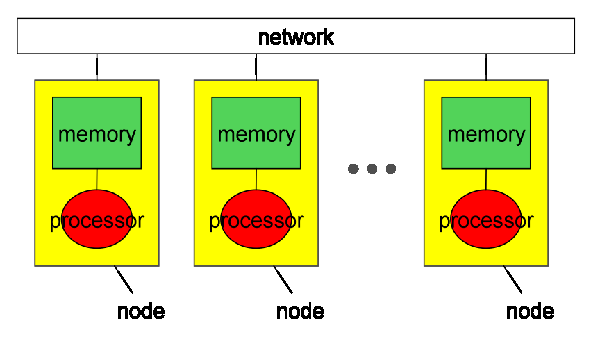
\includegraphics[width=12cm]{figs/Fig1.eps}
  \caption{Hardware Model}\label{fig1}
\end{myfigure}

\section{Execution Model}

An {\XMP} program execution is based on the Single Program Multiple Data
(SPMD) model, where each node starts execution from the same main
routine and keep executing the same code independently
(i.e. aynchronously), which is referred to as the {\it \Term{duplicate
execution}}, until it encounters any {\XMP} directive.

%The basic execution model of {\XMP} is a Single Program Multiple Data
%(SPMD) model on distributed memory. In each node, a program starts from
%the same main routine.
%
%Unless the nodes encounter some {\XMP} directives, they executes the same
%code locally (i.e. aynchronously), which is referred to as
%{\it \Term{duplicate execution}}.

%An {\XMP} program begins as a single thread of
%execution in each node. 

When a node encounters a {\tt loop} or an {\tt array} construct, it
executes the loop or the array assignment in parallel with other nodes,
so that each iteration of the loop or element of the computation is
executed by the node where the specified data element is located.
%
When a node encounters a synchronization or a communication directive,
synchronization or communication occurs between it and other nodes.
%
That is, such ``global constructs'' are performed collectively by the
nodes in the executing node set.
%
Note that nither synchronizations nor communications occur without these
constructs specified.

%In this case, the
%program performs duplicate execution of the same program on local memory
%in each node.

%{\OMP} API can be used in order to make use of multicores in a node. In
%this specification, we define actions only when {\XMP} directives are
%executed one thread at a time.

A set of the nodes that are executing a subprogram, a statement, a loop,
a block, etc. is referred to as its {\it executing node set} and
determeined by the innermost {\tt task} or {\tt loop} directive
surrounding it dynamically.
%
The initial executing node set (or the {\it entire node set}) at the
beggining of the program execution is the set of all available nodes,
which can be specified in a implementation-dependent way (e.g. a
command-line option).

\section{Data Model}

%By default, data declared in the program are allocated in each node and
%are referenced locally by threads executed in the node. 

There are two classes of data in {\XMP}: {\it \Term{global data}} and
{\it local data}. Data declared in a program are local by default.

Global data are ones that are distributed onto the executing node set by
the {\tt align} directive (see section \ref{sub:align}). Each fragment
of a global data is allocated in the local memory of a node in the
executing node set.
%
%In contrast to a local-view programming model, a global-view programming
%model is a model in which programmers express their algorithm and data
%structure in their entirety, mapping them to the node set. The
%programmers describe the data distribution and the work mapping in order
%to express how to distribute data and share the workload among
%nodes. The variables in the global-view programming model appear as a
%shared memory spanning the nodes.
%
Local data are all of the ones that are not global. They are duplicated
in the local memory of each node in the executing node set.

%{\XMP} supports two models of data viewing: the global-view programming
%model and the local-view programming model. In the local-view
%programming model, accesses to data in remote nodes are performed
%explicitly by language extension for get/put operations on remote nodes
%with the node number of the target nodes, while reference to local data
%is executed implicitly.

A node can access directly only a local data and a region of global data
that are allocated in its local memory.
%
To accesse the data in remote memory, explicit communication must be
specified in some ways, such as global comuunication constructs and
coarray assignment.


\section{Global-view Programming Model}

The global-view programming model is useful when, starting from
sequential version of a program, the programmer parallelizes it in
data-parallel style by adding directives incrementally with minimum 
modification.
%
In the global-view programming model, the programmer describes the data
distribution of the data shared among the nodes using the data
distribution directives.
%
The {\tt loop} construct assigns each iteration of a loop to the node
where the computed data is located. 
%
Global-view communication directives are used for synchronization
between nodes, to maintain the consistency of the shadow area, and to
move part of the distributed data globally.
%
Note that the programmer must specify explicitly communications to make
all data referrence in the program local by using appropriate directives.
%Note that the programmer must perform all computations that require data
%reference locally by any appropriate directives.

In many cases, the {\XMP} program according to the global-view
programming model is based on a sequential program and can produce the
same results regardless of the number of computation nodes (Figure
\ref{fig2}).
%The global view provides a 
%programming model in which computation and data are distributed onto
%computation nodes.

There are three groups of directives for the global-view programming
model. Since these directives are ignored as a comment by the
compilers of base languages ({\C} and {\Fort}), an {\XMP} program can be
compiled by them and run rightly.

%an  {\XMP} program derived from a sequential program can preserve the
%integrity of the original program when the program is run sequentially. 

\subsubsection*{Data Mapping}
Specifies the data distribution and mapping to nodes (partially
inherited from HPF).

\subsubsection*{Work Mapping (Parallelization)}
Assigns a work to a node set. The {\tt loop} construct maps each iteration of
a loop to nodes containing the referenced data elements. The {\tt task}
construct creates an amount of work (called a {\it task}) and assigns it
to a node set.

\subsubsection*{Communication and Synchronization}
Describes how to communicate and synchronize with the other compute
nodes. In {\XMP}, inter-node communication must be described
explicitly. The compiler guarantees that no communication occurs
unless it is explicitly specified by the programmer.

\begin{myfigure}
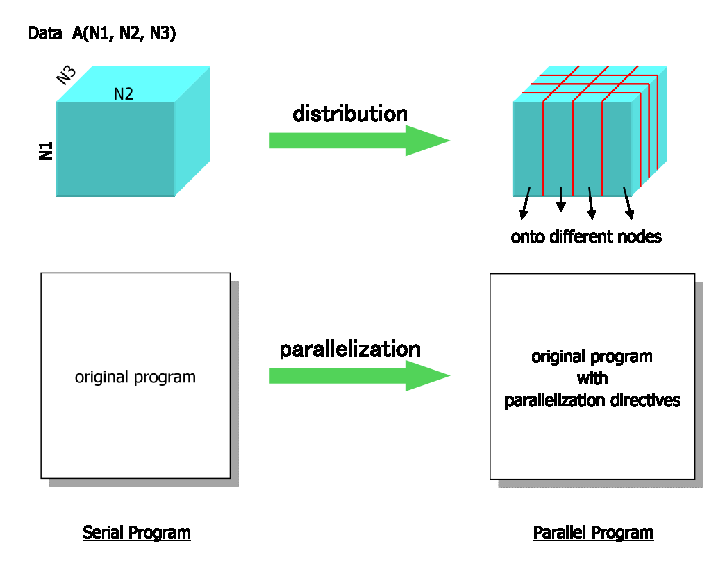
\includegraphics[width=12cm]{figs/Fig2.eps}
  \caption{Parallelization by the global-view programming model}
\label{fig2}
\end{myfigure}

\section{Local-view programming model}

The local-view programming model is suitable for programs that
explicitly describe the algorithm of each node and explicit remote
data reference (Figure \ref{fig3}). Since MPI is based on the local-view
model, the local-view programming model of {\XMP} has high
interoperability with MPI.

For the local-view programming model, some language extensions and 
directives are provided. The coarray notation imported from {\CAF} (CAF)
is such an extension. For example, the expression of {\tt A(i)[N]} is
used to access an array element of {\tt A(i)} located on compute node
{\tt N}.
%
If the access is a reference, then communication to obtain the value
(i.e. get operation) occurs. If the access is a definition, then
communication to set a new value (i.e. put operation) occurs.

\begin{myfigure}
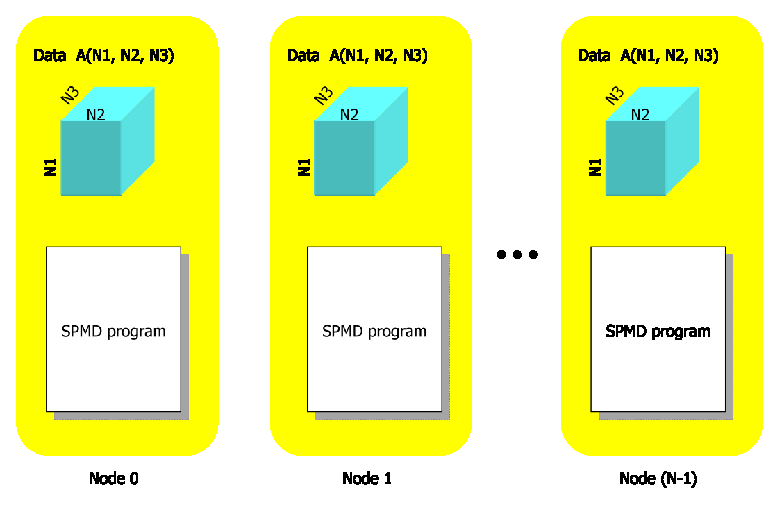
\includegraphics[width=12cm]{figs/Fig3.eps}
  \caption{Local-view programming model}
\label{fig3}
\end{myfigure}

\section{Interactions between the global view and the local view}

In the global view, nodes are used to distribute data and computational
load. In the local view, nodes are used to addresse data in the coarray
notation.
%
In the application program,
programmers should choose an appropriate data model according to the
structure of the program. Figure \ref{fig4} illustrates the global view
and the local view of data.

Data may have both a global view and a local view, and can be accessed
from either. {\XMP} provides some directives to give the local name
(alias) to the global data declared in the global-view programming model
so that they can also be referenced in the local-view programming
model. This feature is useful to optimize a certain part of the program
by using explicit remote data reference in the local-view programming
model.

\begin{myfigure}
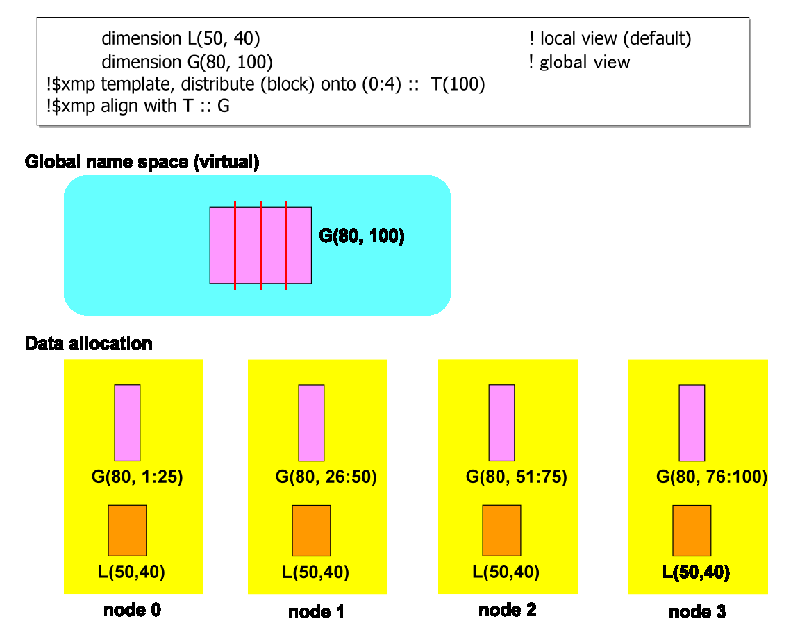
\includegraphics[width=12cm]{figs/Fig4.eps}
  \caption{Global view and local view}
\label{fig4}
\end{myfigure}

%\section{Execution model and task}
%
%
%In {\XMP}, a program begins as a single thread
%of execution in each node. The set of nodes when starting a program is
%referred to as the entire node set.
%
%A task is a specific instance of executable
%code and its data environment executed in a set of nodes. A task when
%starting a program in the entire node set is called an initial task. The
%initial task can generate a subtask, which is executed on a subset of the
%nodes by the {\tt task} construct. A set of nodes executing the same task is
%referred to as the set of executing nodes. If no {\tt task} construct is encountered, then a
%program is executed as a single task, and its executing nodes are the entire node set.
%
%If no directives are encountered, then a program is executed
%locally. When the same codes are executed, almost the same computation is
%performed in each node, which is referred to as duplicate execution. When the threads
%encounter a {\tt loop} construct or an {\tt array} construct, the specified
%loop is executed in parallel, so that each iteration is assigned to the
%node where the specified data element is located. 
%
%A new task is generated by
%the {\tt task} construct. A code in the {\tt task} construct is executed
%as a subtask executed in a specified node set. When a subroutine is
%called in the context of the task, the subroutine is executed on its
%executing nodes. 
%
%For synchronization and communication between nodes, a set of
%directives is provided. In the local-view programming model, coarray
%features are adopted for remote data reference. Note 
%that all synchronization and communication are specified explicitly by directives, and without such directives, no communications are
%executed implicitly by the compiler.
